\chapter{Baseline Supervisionate e Protocollo di Sample Efficiency}
\label{chap:sample_efficiency}

\section{Obiettivo e Disegno Sperimentale}
\label{sec:sample_disegno}
La domanda di ricerca che guida il confronto è:
\begin{quote}
    \centering
    \textit{<<A quale frazione di dati annotati manualmente con bounding box equivale un modello addestrato senza alcuna annotazione geometrica supervisionata?>>}
\end{quote}

Per misurare questo rapporto in modo controllato, è stato impostato il protocollo di \textit{sample efficiency} illustrato nella Figura~\ref{fig:protocollo_sample_efficiency}. Il modello YOLOv8n distillato ($0\%$ di coordinate supervisionate) viene confrontato con rilevatori identici addestrati su frazioni progressive di etichette reali (\textit{ground truth}).

\begin{figure}[htbp]
\centering
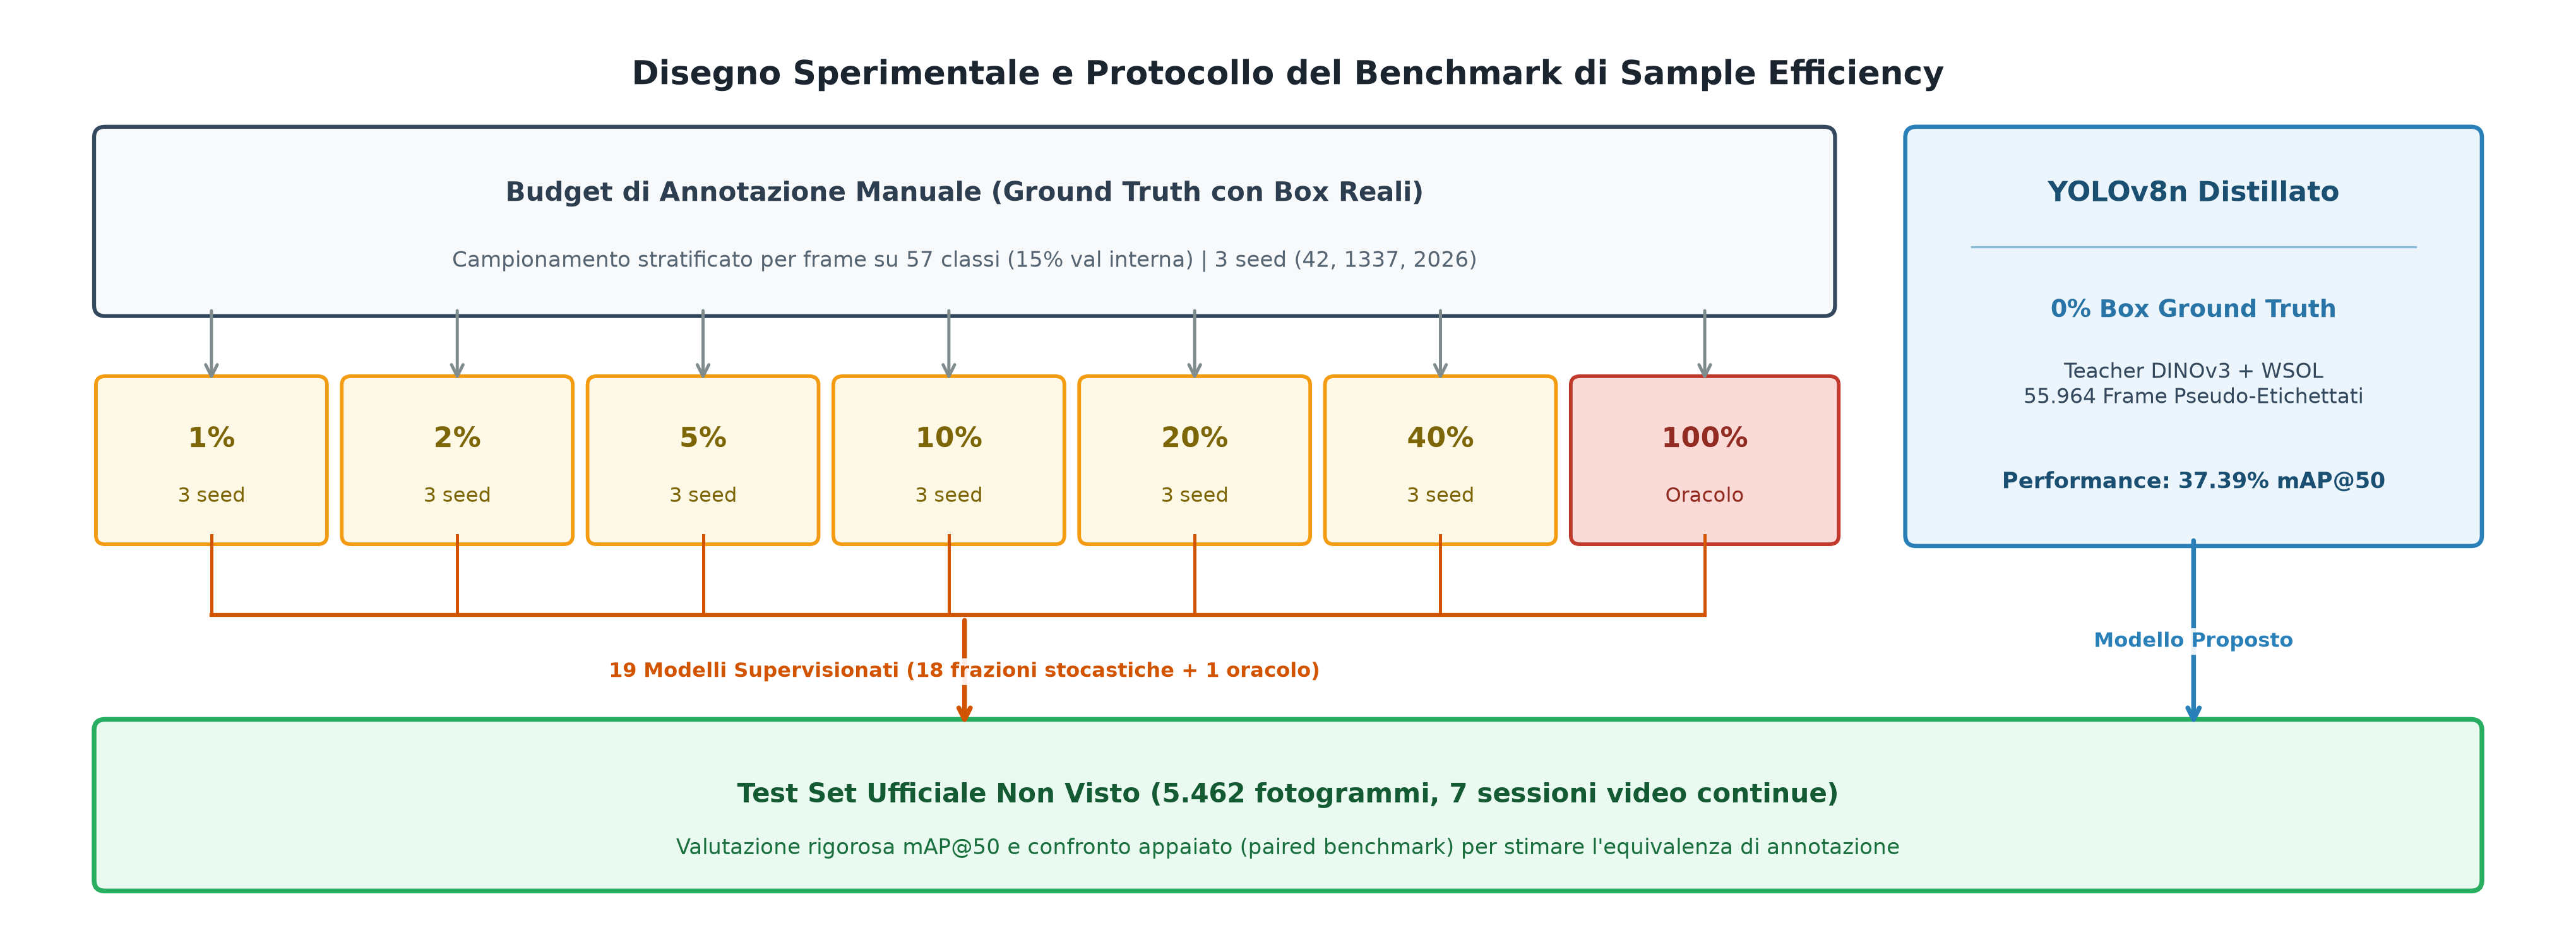
\includegraphics[width=0.92\textwidth]{figure/protocollo_sample_efficiency.png}
\caption{Disegno sperimentale del benchmark di Sample Efficiency: partizionamento stratificato del budget di annotazione umana su 7 frazioni (con 3 repliche stocastiche e validazione interna), confrontato con lo studente distillato sul test set ufficiale non visto.}
\label{fig:protocollo_sample_efficiency}
\end{figure}

\subsection{Frazioni di campionamento e controllo della varianza}
La curva di apprendimento supervisionata è stata campionata su sette quote:
\begin{equation}
    \mathcal{F} = \{1\%, \, 2\%, \, 5\%, \, 10\%, \, 20\%, \, 40\%, \, 100\%\}
\end{equation}
Per le frazioni inferiori al $100\%$ sono stati adottati tre criteri sperimentali:
\begin{itemize}
    \item \textbf{Stratificazione per classe}: la quota $\alpha \in \mathcal{F}$ è calcolata sul numero di immagini di ciascuna delle 57 classi, rispecchiando una campagna di etichettatura bilanciata.
    \item \textbf{Tre seed stocastici}: per limitare la varianza campionaria a bassi volumi di dati, gli addestramenti sotto il $100\%$ sono stati eseguiti su 3 seed casuali ($\text{seed} \in \{42, 1337, 2026\}$) con disegno a blocchi appaiati, calcolando media e deviazione standard ($\mu \pm \sigma$).
    \item \textbf{Validazione interna ($15\%$)}: ogni partizione riserva il $15\%$ dei fotogrammi all'early stopping e alla scelta del miglior checkpoint, senza toccare il test set esterno.
\end{itemize}

\section{Metriche di Valutazione e Condizioni di Fairness}
\label{sec:sample_metriche}
Tutti i modelli sono valutati sul test set ufficiale ($5.462$ immagini, con $3.673$ annotazioni di POI su 7 sessioni continue). Le metriche registrate sono mAP@50 ($\text{IoU} \ge 0.50$), mAP@50:95 (media integrale su soglie da $0.50$ a $0.95$ a passo $0.05$) e le prestazioni suddivise per tier dimensionale.

Per isolare l'effetto della quantità di dati ed evitare discrepanze esterne, i modelli condividono la medesima impostazione:
\begin{enumerate}
    \item \textbf{Architettura}: YOLOv8n ($3.2\text{ M}$ parametri, $8.7\text{ GFLOPs}$) per ogni configurazione.
    \item \textbf{Inizializzazione}: pesi pre-addestrati COCO rilasciati da Ultralytics.
    \item \textbf{Condizioni di addestramento}: risoluzione $640 \times 640$, ottimizzatore SGD con momentum ($0.937$), weight decay $5 \times 10^{-4}$, funzione di perdita comune (BCE + CIoU + DFL), massimo 100 epoche e stessa data augmentation (Mosaic, HSV, flip).
    \item \textbf{Test set intatto}: nessun fotogramma di test è stato utilizzato per calibrazione o regolazione degli iperparametri.
\end{enumerate}
